\documentclass{article}

% if you need to pass options to natbib, use, e.g.:
% \PassOptionsToPackage{numbers, compress}{natbib}
% before loading nips_2018

% ready for submission
% \usepackage{nips_2018}

% to compile a preprint version, e.g., for submission to arXiv, add
% add the [preprint] option:
\usepackage[preprint]{nips_2018}

% to compile a camera-ready version, add the [final] option, e.g.:
% \usepackage[final]{nips_2018}

% to avoid loading the natbib package, add option nonatbib:
% \usepackage[nonatbib]{nips_2018}

\usepackage[utf8]{inputenc} % allow utf-8 input
\usepackage[T1]{fontenc}    % use 8-bit T1 fonts
\usepackage{hyperref}       % hyperlinks
\usepackage{url}            % simple URL typesetting
\usepackage{booktabs}       % professional-quality tables
\usepackage{amsfonts}       % blackboard math symbols
\usepackage{nicefrac}       % compact symbols for 1/2, etc.
\usepackage{microtype}      % microtypography

\usepackage{amsmath}
\usepackage{graphicx}       % including images
\graphicspath{ {./images/} }
\usepackage{algorithm}
\usepackage{algpseudocode}  % including algorithms

\title{Deep Reinforcement Learning and Transfer Learning with FlappyBird}

% The \author macro works with any number of authors. There are two
% commands used to separate the names and addresses of multiple
% authors: \And and \AND.
%
% Using \And between authors leaves it to LaTeX to determine where to
% break the lines. Using \AND forces a line break at that point. So,
% if LaTeX puts 3 of 4 authors names on the first line, and the last
% on the second line, try using \AND instead of \And before the third
% author name.

\author{
  Cedrick Argueta, Austin Chow, Cristian Lomeli \\
  Department of Computer Science\\
  Stanford University\\
  Stanford, CA 94305 \\
  \texttt{\{cedrick, archow, clomeli\}@cs.stanford.edu} \\
}

\begin{document}
% \nipsfinalcopy is no longer used

\maketitle

\begin{abstract}

Reinforcement learning's growth in popularity in recent years is partly due to its ability to play some video games with a level of mastery that no human can reach. 
Transfer learning is popular in the field of deep learning, and using pre-trained models on certain tasks speeds up training time and increases performance significantly. 
In this project we aim to apply transfer learning to the popular video game \textit{FlappyBird} and analyze its performance compared to traditional reinforcement learning algorithms.
 
\end{abstract}


\section{Introduction}
Reinforcement learning is a technique for solving certain decision tasks, where an agent attempts to maximize a long-term reward through trial and error. 
This trial and error paradigm is better explained through the lens of exploration and exploitation: the agent must decide whether it explores and learns new information, or exploits the current policy to maximize reward.
We will primarily explore the applicability of deep Q-learning, a deep reinforcement learning algorithm, to the FlappyBird game.
In addition, we intend to explore the impact of transfer learning, a machine learning technique where a model developed for a specific task is reused as the starting point for a model in a second task. 
Being able to transfer learn will allow us to develop a more general model for different tasks, saving time and effort.
In particular, we aim to see whether transfer learning will speed up training time to reach the same performance level as the DQN model.

\section{Literature Review}
The impetus behind our project is DeepMind's paper, "Playing Atari with Deep Reinforcement Learning". Mnih et al. were able to show how a Deep Q-Network could take raw image pixels from an Atari game and estimate the $Q$ function. \cite{deepmind}
Their model also takes advantage of recent advances in convolutional neural networks for image processing, a target network for stabilizing policy updates, and experience replay for a more efficient use of previous experience.
Transfer learning is the idea that generalization occurs both within tasks and across tasks. \cite{transfer}
Deep reinforcement learning may benefit from transfer learning, especially since convolutional neural networks are often used for playing games.
Since convolutional neural networks often learn similar features in the first, second, etc. layers across a range of image classification tasks, it's possible that transfer learning in the context of reinforcement learning for video games can exploit this.

\section{Game Mechanics}

The game of FlappyBird can be described as follows: a bird flies at a constant horizontal velocity $v_x$ and a variable veritcal velocity $v_y$. 
The bird can flap its wings, giving it a boost in altitude and velocity $v_y$.
The aim of the game is to avoid randomly generated pipes that restrict the flying area, leaving only a small gap for the bird to fly through. 

We model the problem as a Markov decision process with no knowledge of the transition probabilities or reward function at every state.
The transition probabilities are unknown, since each state consists of the deterministic bird position and velocity, along with the non-deterministic pipe positions.
The only reward signal received from the game in its standard implementation is when the bird flies past a pipe, giving us a reward of $1$. 
This sparse reward makes it impossible for us to get an explicit reward for each $(s, a, s')$ tuple.
The start state $s_{start}$ is the bird at some constant height, with no pipes on the screen.
The actions for every state are the same: the bird can flap its wings or not.
The only exception to this are the end states $s_{end}$, where the bird collides with a pipe or the ground.
In these cases, there are no actions to take, and the episode ends.

We have a similar model for \textit{PixelCopter}, the game we plan on transfer learning with.
These games are similar in terms of objective and action/observation spaces, so we hope that by applying transfer learning we are able to speed up training time and perhaps maximum absolute reward.

\section{Approach}

The goal of our project is twofold: we aim to evaluate deep reinforcement learning algorithms on the FlappyBird game, and also experiment with transfer learning to analyze the impact it makes on the training process. 

Vanilla learning methods like Q-learning are not well suited to this problem, since the state space of the game is very large. The position of the bird and pipes are continuous values, and as such we have an almost-zero probability of reaching a particular state that we've seen before.
Thus, it will be necessary to use either function approximation to generalize to unseen states or some form of deep learning that can extract features automatically.
We envision using Deep Q-networks as a nice foray into deep learning, given our experience with Q-learning.
The DQN model uses a neural network to approximate the Q action-value function, and allows for better generalization than the standard Q-learning approach.

Furthermore, we will demonstrate the ability for policies learned through deep reinforcement learning on  other games to transfer to FlappyBird.
This has been demonstrated before, particularly through the use of convolutional neural networks for playing games directly from pixels. \cite{deepmind}
In our case specifically, we will develop a Q-network parameterized by weights $\theta_{FlappyBird}$ that performs `well enough' on FlappyBird, along with Q-networks parameterized by $\theta_{PixelCopter}$ that perform `well enough' on the game PixelCopter.
These networks will be initialized through Xavier initialization. \cite{xavier}
Once we have this, we will begin training new Q-networks parameterized by $\theta'_{PixelCopter}$ that were initialized with $\theta_{FlappyBird}$.
We do this by fixing weights up until the final hidden layer, and solely training those weights.
This gives the effect of reducing the number of parameters needed for optimization, making our training faster and more efficient.
We will then compare the training times and absolute performance of the $\theta$ and $\theta'$ models, demonstrating the increase in efficiency or performance that transfer learning entails.

\subsection{Infrastructure}

The infrastructure for the game comes mostly from the PyGame Learning Environment, OpenAI gym, and keras-rl packages. 
The PyGame Learning Environment provides a nicely wrapped implementation of FlappyBird, complete with sprites and the relevant game mechanics built in. \cite{ple} \cite{openaigym} \cite{ale}
Keras-rl provides a deep reinforcement learning framework that gives us a simple interface for training agents. 
We take advantage of these two here, writing simple wrappers for the PLE game instance so that it is compatible with keras-rl. \cite{kerasrl}
The keras-rl package additionally provides an implementation of several algorithms that are applicable to FlappyBird, particularly Deep Q-networks and the SARSA algorithm.
For the transfer learning portion of the project, we saved weights info \texttt{hdf5} files with the Keras package.
The neural networks and much of the other deep learning architecture was also created in Keras, with a TensorFlow backend. \cite{keras} \cite{tensorflow}
This allowed us to monitor training time and other metrics inside TensorBoard.

Code for our project can be found at this link: \href{https://github.com/cdrckrgt/cs221-project} {https://github.com/cdrckrgt/cs221-project}.

\section{Model}

In this section, we describe the DQN algorithm and how it applies to our task. We use a modified version of the algorithm described in the 2013 DeepMind paper.

Again, we model the environment $\mathcal{E}$ as a Markov decision process with no knowledge of the transition probabilities or reward function at every state.
There is a set of actions that may be taken at every time-step, designated $\mathcal{A}$.
Each interaction between the agent and its environment at time $t$ produces an observation $x_t \in \mathbb{R}^{d}$ and reward $r_t$, where $d$ is the dimensionality of the environment.

As in the standard Q-learning algorithm, we consider sequences of observations, actions, and rewards $x_1, a_1, r_1, \dots, x_t, a_t, r_t$ as the state of $\mathcal{E}$ at time $t$. 
The objective of the agent is to maximize its future reward, defined as:
\begin{equation}
\displaystyle R_t = \sum_{t' = t}^{T} \gamma^{t' - t}r_{t'}
\end{equation}
such that $T$ is the termination time-step of the game.
Then the optimal Q-value function is defined as follows:
\begin{equation}
\displaystyle Q^{*}(s, a) = \max_{\pi}\mathbb{E}[R_t\ |\ s_t = s, a_t = a, \pi]
\end{equation}
such that $\pi$ is a policy that maps states to actions.
So far we have described steps to arriving at the Q-learning algorithm described by Dayans and Watkins. \cite{qlearning} 
The DQN algorithm presented by DeepMind makes numerous improvement on this algorithm by introducing a non-linear function approximator and experience replay.

\subsection{The Q-network}
Since the vanilla Q-learning algorithm does not generalize well to state spaces as large as those encountered in video games, we use a neural network to approximate the Q-value function. 
Then we have a neural network parametrized by weights $\theta$ such that $Q(s, a; \theta) \approx Q^{*}(s, a)$.
At every iteration of training $i$, we minimize the squared error between the current Q-function and the optimal Q-function, according to the loss function:
\begin{equation}
\displaystyle L_i(\theta_i) = \mathbb{E}_{s, a \sim \rho(\cdot)}[(y_i - Q(s, a; \theta_i))^2]
\end{equation}
where $y_i = \mathbb{E}_{s' \sim \mathcal{E}}[r + \gamma\max_{a'}Q(s', a'; \theta_{i - 1}\ |\ s, a]$ and $\rho(s, a)$ is a probability distribution over states and actions. 
The intuition behind this loss function is that we are minimizing the distance between our target, which is the maximum expected future reward for this state and the previous iteration's weights, and our current Q value.
We are effectively getting closer and closer to the true Q values every training iteration.
To minimize this objective function, we update the weights according to the gradient:
\begin{equation}
\displaystyle \nabla_{\theta_i}L_i(\theta_i) = \mathbb{E}_{s, a \sim \rho(\cdot)}[(r + \gamma \max_{a'}Q(s', a'; \theta_{i - 1}) - Q(s, a; \theta_i))\nabla_{\theta_i}Q(s, a; \theta_i)]
\label{eq:gd}
\end{equation}
And we've now arrived at the Deep Q-network algorithm that we can apply to our task.
It's important to note that the original DQN paper applies this algorithm to raw pixel vectors as each $x_t$, whereas we use the internal game state for each $x_t$.
This allows us to achieve the same level of performance in a much quicker fashion, since we don't need to spend the extra compute power on training a convolutional neural network to learn features for each game.
The algorithm, lifted from Mnih's paper, is described in \ref{alg:dqn}.

\begin{algorithm}
\caption{Deep Q-learning with Experience Replay}
\label{alg:dqn}
\begin{algorithmic}[1]
\State Initialize replay memory $\mathcal{D}$ to capacity $N$
\State Initialize action-value function $Q$ with random weights
\For{$\textrm{episode} = 1, M$}
    \State Initialize sequence $s_1 = \{x_1\}$ and preprocessed sequenced $\phi_1 = \phi(s_1)$
    \For{$t = 1, T$}
        \State With probability $\epsilon$ select a random action $a_t$
        \State otherwise select $a_t = \max_{a}Q^{*}(\phi(s_t), a; \theta)$
        \State Execute action $a_t$ in emulator and observe reward $r_t$ and observation $x_{t + 1}$
        \State Set $s_{t + 1} = s_t, a_t, x_{t + 1}$ and preprocess $\phi_{t + 1} = \phi(s_{t + 1})$
        \State Store transition $(\phi_t, a_t, r_t, \phi_{t + 1})$ in $\mathcal{D}$
        \State Sample random minibatch of transitions $(\phi_j, a_j, r_j, \phi_{j + 1})$
        \State Set $ \displaystyle  y_j = 
                        \begin{cases}
                            r_j & \textrm{for terminal}\ \phi_{j + 1} \\
                            r_j + \gamma\max_{a'}Q(\phi_{j + 1}, a'; \theta) & \textrm{for non-terminal}\ \phi_{j + 1} \\
                        \end{cases}
                   $
        \State Perform a gradient descent step on $(y_j - Q(\phi_j, a_j; \theta))^2$ according to equation \ref{eq:gd}
    \EndFor
\EndFor
\end{algorithmic}
\end{algorithm}

\subsection{Experience Replay}
Additionally, the algorithm presented in Mnih's paper makes use of experience replay to smooth learning and prevent divergence.
Rather than performing gradient updates on each consecutive sample, samples are stored in a ring buffer and sampled randomly during the learning phase of the algorithm. 
This has the effect of improving sample efficiency and removing the dependence of each training update on the previous training update.

\subsection{Target Network}
Finally, we make use of a target network to further stabilize the training process. 
Note that during our gradient descent, the weights that produce our target values shift every iteration.
Instead of using these rapidly shifting weights, we copy the parameters of the training network $\theta_{training}$ to a second, identical model $\theta_{target}$.
With this identical model, we may compute the same targets, albeit with less variance by only updating the $\theta_{target}$ to match the $\theta_{training}$ with some fixed, low probability at every iteration.

\subsection{Annealed $\epsilon$-greedy Policy}
Rather than use the standard $\epsilon$-greedy policy, we opted to use a policy that annealed $\epsilon$ from some value $\alpha$ to some value $\beta$ over training.
Our goal was to incentivize exploration early on, but revert back to the usually $\epsilon$-greedy policy after some about of training.


\subsection{Model Architecture}
Since we use as input to the Q-network the internal game state representation as opposed to the raw pixel inputs, we don't make use of a convolutional neural network to learn features directly from the game's pizels.
We instead make use of a multi-layered perceptron that takes as input the game's state in vector form.
In the case of FlappyBird, the state vector is a vector in $\mathbb{R}^8$, and contains the bird's position, velocity, and the distance, top, and bottom positions of the next two pipes.
The dimensionality of the input differed for each game we worked with, but we kept the dimensionality of the hidden layers the same for each game so that we could experiment with transfer learning.
We have three fully connected hidden layers, with dimensionality 256, 128, and 16.
The outputs of the Q-network for each game were the Q-values of all actions in the action space for that game.
In the case of FlappyBird, the output was two Q-values in $\mathbb{R}$, one for the action to jump, and the null action.

\section{Results}

\subsection{Vanilla DQN}
After finalizing the implementation of the DQN algorithm, we experimented with different hyperparameters and had to define performance metrics to compare the base DQN models with the transfer learned models. 
The hyperparameters for the models trained from scratch are shown in table \ref{hyperparams-xavier}.
We see in the graph \ref{fig:flappy-training-eps} the variance in episode reward over different random seeds for the FlappyBird game.
Each run was trained for 30,000 iterations, and we see the ability for DQN to learn to play the game sometimes but fail other times.
We aim to decrease this variance soon through more hyperparameter optimization and tinkering with the model architecture more.
The DQN performs well above the ability of the average human when it does learn to play the game, since it can sometimes average scores in the thousands while testing.

\begin{table}[h!]
\centering
\begin{tabular}{ll}

\multicolumn{2}{ c }{ \textbf{Hyperparameters for Xavier-initialized networks} } \\

\\

    \begin{tabular}{| c | c |}
    \hline
    \multicolumn{2}{| c |}{FlappyBird Hyperparameters} \\ 
    \hline
    Target Model Update & 1e-2 \\
    \hline
    Learning Rate & 1e-3 \\
    \hline
    $\gamma$ & 0.99 \\
    \hline
    Annealed $\epsilon$ & 0.4 $\rightarrow$ 0.1 \\
    \hline
    \multicolumn{2}{| c |}{Reward Profile} \\ 
    \hline
    tick & $0.1$ \\
    \hline
    passed pipe & $1.0$ \\
    \hline
    collided & $-10.0$ \\
    \hline
    \end{tabular}

&

    \begin{tabular}{| c | c |}
    \hline
    \multicolumn{2}{| c |}{PixelCopter Hyperparameters} \\ 
    \hline
    Target Model Update & 1e-1 \\
    \hline
    Learning Rate & 1e-3 \\
    \hline
    $\dots$ & $\dots$ \\
    \hline
    tick & $0.1$ \\
    \hline
    passed block & $1.0$ \\
    \hline
    collided & $-10.0$ \\
    \hline
    \end{tabular}

\\

\end{tabular}
\caption{These hyperparameters were obtained with lots of trial and error. If not noted here, the hyperparameter was left as the default value in Keras.}
\label{hyperparams-xavier}
\end{table}

\begin{figure}[h!]
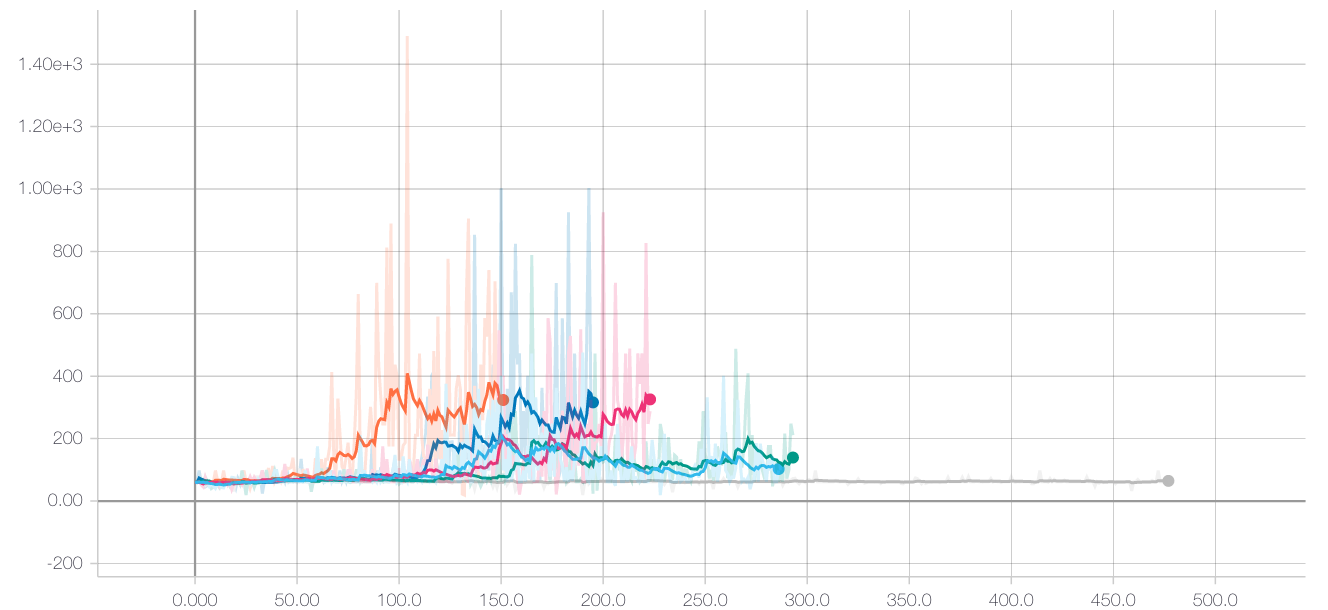
\includegraphics[width=\textwidth]{flappy-training-eps}
\label{fig:flappy-training-eps}
\caption{6 different runs for DQN on FlappyBird. The x-axis shows episode number, while the y-axis shows episode length.}
\end{figure}

\begin{figure}[h!]
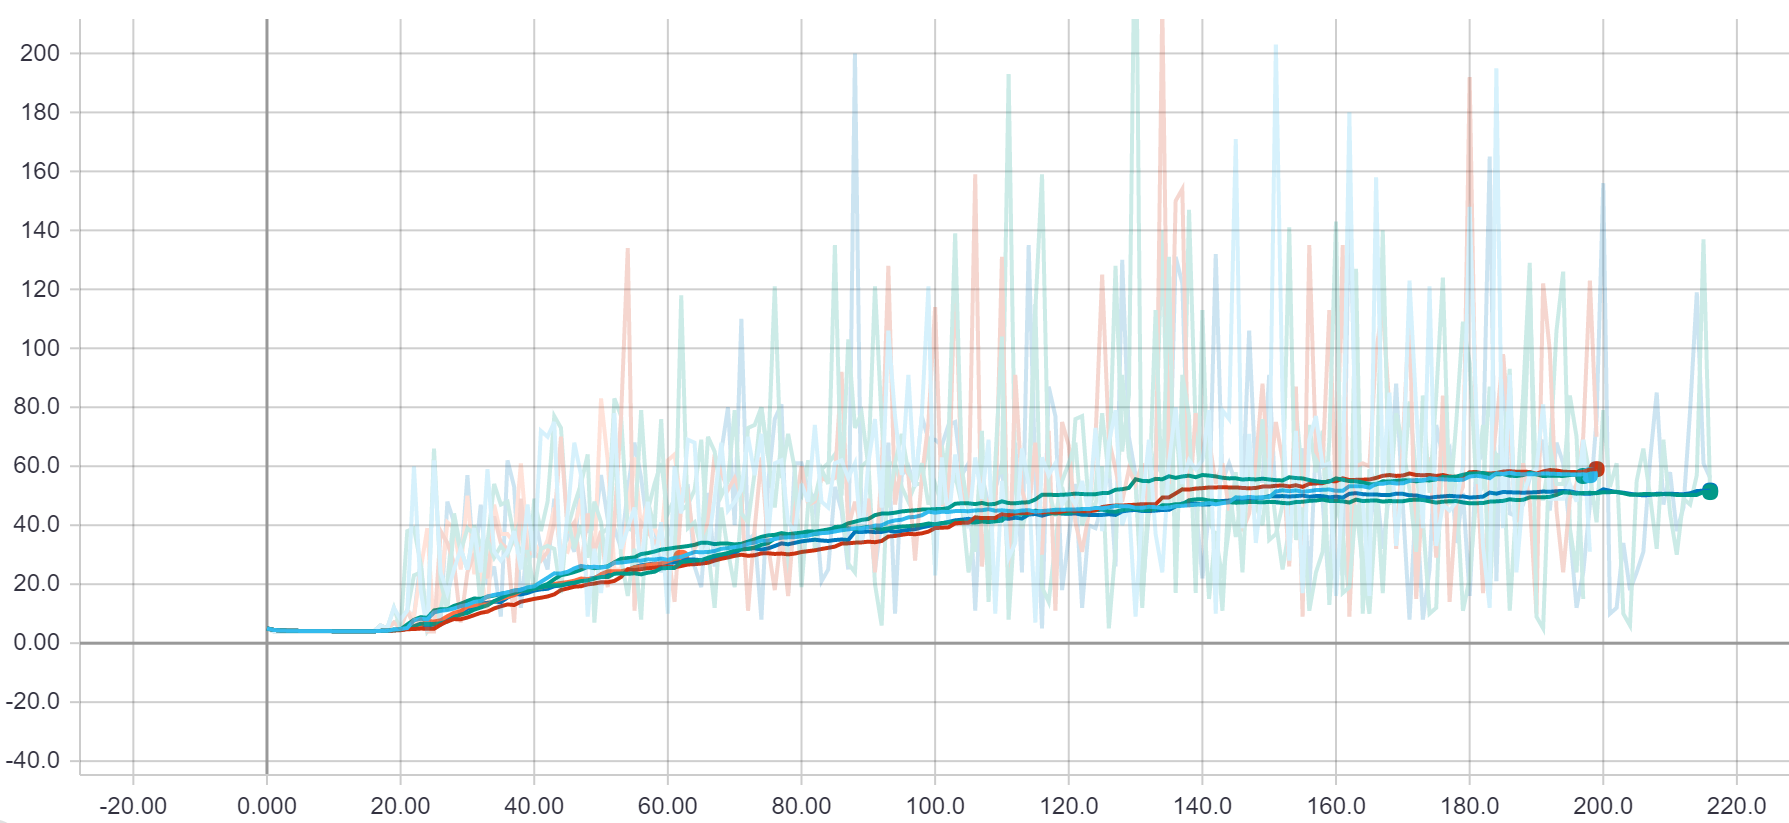
\includegraphics[width=\textwidth]{pixelcopter-training}
\caption{5 different runs for DQN on PixelCopter. The x-axis shows episode number, while the y-axis shows episode length.}
\label{fig:other-training}
\end{figure}
We show the performance of the DQN trained on the PixelCopter training in \ref{fig:other-training}.
For both games, we show the episode length as a proxy for how good the agent performs on the episode.
The performance of DQN on PixelCopter without transfer learning plateaus very early on, and has a very poor performanc eoverall.

\subsection{Transfer Learning}
We show in \ref{fig:transfer-training} the effectiveness of using pre-trained weights from FlappyBird on the game PixelCopter.

\begin{figure}[h!]
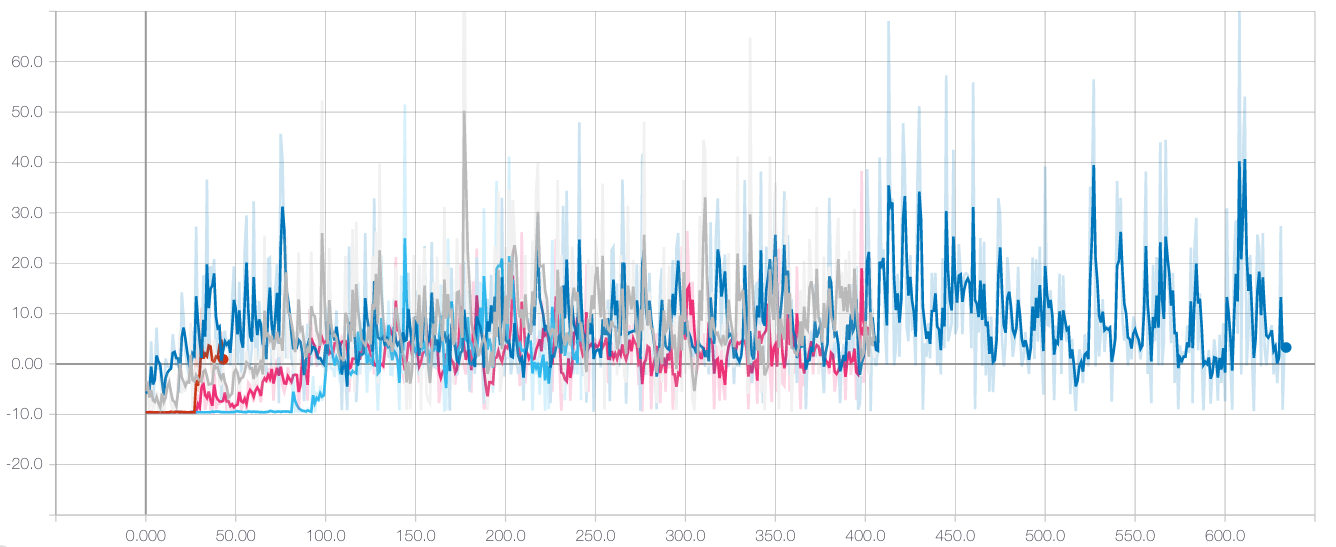
\includegraphics[width=\textwidth]{pixelcopter-transfer}
\label{fig:transfer-training}
\caption{6 different runs for the DQN on PixelCopter, using weights pretrained on FlappyBird.}
\end{figure}


\subsection{Analysis}
We are still working out the kinks from transfer learning with solely dense layers. 
One of the approaches we may try is just changing the input from the state vector representation to the image, since convolutional neural nets have been shown to transfer learn well with CNNs.
The traditional method of freezing some subset of middle layers and only training the outer layers hasn't proved effective so far.

Additionally, we have yet to begin training on machines stronger than our laptops.
Because of this, we've haven't been able to practically train for periods of longer than 50,000 iterations.
Because of the nature of some of these games, it might take longer than that to see some improvement, especially if we were to generalize the DQN to receieve images as input.
Despite this, we were still able to get some good results on the vanilla DQN and FlappyBird.

The vanilla DQN model trained on PixelCopter doesn't generally perform well, even with long training times and hyperparameter tuning.
Our hypothesis is that the state vector that the game produces doesn't yield enough information about the game for the model to learn how to play. 
Only the wall directly above and below the Pixelcopter is shown to the model, leaving the rest of the terrain unknown until the PixelCopter flies past it.
One way to approach this issue is to simply feed the pixel representation of the game's state as image input to the model, which would necessitate the use of CNNs.

Because the performance of DQN on PixelCopter was poor to begin with, we hoped to achieve better results through transfer learning.
After running tests with transfer learning, we see similar performance to the non-transfer-learned DQN model on PixelCopter, leading us to believe that the transfer learning was ineffectual.
We don't know the effectiveness of transfer learning on solely fully-connected layers, and hopefully this goes to show us that we might want to continue with CNNs and learning from pixel input in the future.



\section{Results}


in here is just the presentation of our results, no analysis yet.
include in here stuff like graphs, numbers, descriptions of how the agent trained and performed, even stuff like anecdotes/empirical evidence about where the model would fail or succeed particularly badly/well

\subsection{DQN on FlappyBird}

\subsection{DQN on PixelCopter}

\subsection{Transfer Learning on PixelCopter}

\section{Analysis}

include in here our rationalization of our results
stuff like: how a particular model design decision influenced the results of our model, why we think that an agent performed well or poorly on some stuff, speculation on what could be done to improve the model, 

\subsection{Effectiveness of Feature Engineering}

\subsection{Effectiveness of Transfer Learning}

\subsection{Model Architecture Considerations}

\subsection{Expansion to Pixel Inputs}

\section{Conclusion and Future Work}


\bibliography{ref}
\bibliographystyle{plain}


\end{document}

